\documentclass[conference]{IEEEtran}
\usepackage{tikz}
\usetikzlibrary{arrows.meta,positioning,shapes.geometric,fit,calc,decorations.pathreplacing,chains}
\usepackage{booktabs}
\usepackage{enumitem}
\usepackage{xcolor}
\usepackage{hyperref}
\usepackage{listings}
\usepackage{caption}
\usepackage{float}
\usepackage{balance}
\usepackage{tabularx}
\usepackage{array}
\usepackage{amsmath}

\hypersetup{colorlinks=true, linkcolor=blue!70!black, urlcolor=blue!70!black}

\definecolor{accent}{HTML}{C2410C}
\definecolor{accentlight}{HTML}{FFF7ED}
\definecolor{secondary}{HTML}{7C3AED}
\definecolor{success}{HTML}{16A34A}
\definecolor{err}{HTML}{DC2626}
\definecolor{txt}{HTML}{1C1917}
\definecolor{txt2}{HTML}{78716C}
\definecolor{bluea}{HTML}{2563EB}
\definecolor{l1}{HTML}{EAB308}
\definecolor{l2}{HTML}{EA580C}
\definecolor{l3}{HTML}{DC2626}
\definecolor{teal}{HTML}{0D9488}
\definecolor{indigo}{HTML}{4F46E5}
\definecolor{rose}{HTML}{E11D48}
\definecolor{amber}{HTML}{D97706}
\definecolor{sky}{HTML}{0284C7}
\definecolor{emerald}{HTML}{059669}
\definecolor{violet}{HTML}{7C3AED}

\lstset{
  basicstyle=\ttfamily\scriptsize,
  backgroundcolor=\color{gray!5},
  frame=single,
  rulecolor=\color{gray!30},
  breaklines=true,
  columns=fullflexible,
}

\begin{document}

\title{TeachLoop: An AI-Powered Communication Practice Platform for Technical Professionals}

\author{
\IEEEauthorblockN{Belalia Mohamed Oussama}
}

\maketitle

\begin{abstract}
Effective communication of technical concepts is a critical professional skill rarely taught in formal education. This paper presents TeachLoop, a web-based platform that helps engineers practice explaining complex technical topics through AI-powered feedback. The system employs a three-mode architecture (Teaching, Interview, Custom) with audience-aware evaluation across five communication dimensions. A progressive hint system provides scaffolding from gentle nudges to comprehensive explanations, drawing on Vygotsky's Zone of Proximal Development. The platform uses a client-side state machine with localStorage persistence, proxying evaluations to a large language model via a single API route. We describe the system architecture, the AI evaluation pipeline with rate limiting and schema validation, the design system comprising three themes with 40+ CSS custom properties, and accessibility features targeting WCAG AAA compliance. A content database of 36 curated questions with 108 progressive hint sets covers AI/ML concepts and system design topics. TeachLoop demonstrates that effective AI-assisted communication practice can be delivered with zero backend infrastructure beyond the AI proxy.
\end{abstract}

\begin{IEEEkeywords}
communication practice, AI feedback, scaffolding, web application, technical education, progressive hints
\end{IEEEkeywords}

% ══════════════════════════════════════════════════════════
\section{Introduction}
\label{sec:intro}

Software engineers frequently struggle to explain complex systems to non-technical stakeholders, junior developers, or interviewers. While technical knowledge is necessary, the ability to \emph{communicate} that knowledge effectively determines career outcomes---from passing technical interviews to leading cross-functional projects. Studies in engineering education consistently show that communication skill is among the top factors in hiring decisions, yet it is rarely taught in formal curricula~\cite{deeplearning}.

Existing tools focus on technical skill assessment---coding challenges, system design quizzes, flashcards---but neglect the communication dimension entirely. A developer may understand backpropagation deeply but be unable to explain it to a product manager. TeachLoop addresses this gap by evaluating \emph{how} users explain, not merely \emph{what} they know.

The platform presents users with technical concepts (e.g., backpropagation, CAP theorem, transformer architecture, ride-sharing system design) and asks them to explain these concepts to various audiences---from a curious 10-year-old to a senior AI engineer. An AI model evaluates each explanation across five communication dimensions and provides actionable feedback. The system is designed around four explicit principles: coach over critic, focus on the human, progress is visible, and warmth through craft.

Fig.~\ref{fig:userflow} illustrates the complete user journey through the platform, from initial concept selection through AI evaluation and feedback delivery.

\begin{figure}[!t]
\centering
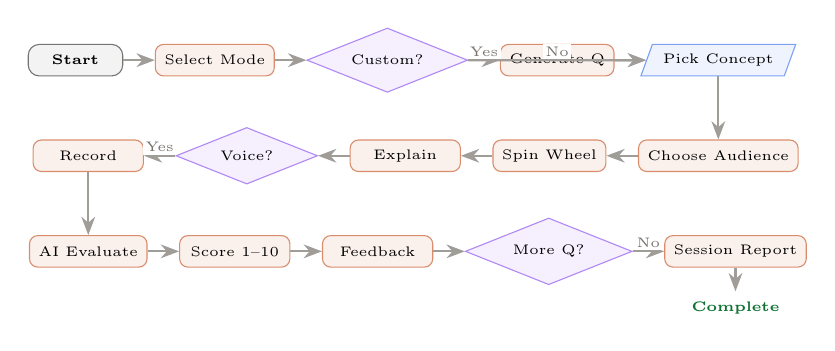
\begin{tikzpicture}[
  >=Stealth,
  node distance=0.5cm,
  startstop/.style={rectangle, rounded corners, minimum width=1.2cm, minimum height=0.4cm, text centered, draw=txt!60, fill=txt!5, font=\tiny\bfseries},
  process/.style={rectangle, minimum width=1.4cm, minimum height=0.4cm, text centered, draw=accent!60, fill=accent!8, font=\tiny, rounded corners=3pt},
  decision/.style={diamond, minimum width=1.2cm, minimum height=0.4cm, text centered, draw=secondary!60, fill=secondary!8, font=\tiny, aspect=2.5},
  io/.style={trapezium, trapezium left angle=70, trapezium right angle=110, minimum width=1.4cm, minimum height=0.4cm, text centered, draw=bluea!60, fill=bluea!8, font=\tiny},
  arr/.style={->, thick, color=txt2!70},
  lbl/.style={font=\tiny, text=txt2, fill=white, inner sep=1pt},
]

\node[startstop] (start) {Start};
\node[process, right=0.4cm of start] (mode) {Select Mode};
\node[decision, right=0.4cm of mode] (custom) {Custom?};
\node[process, right=0.4cm of custom] (genq) {Generate Q};
\node[io, right=0.4cm of genq] (pick) {Pick Concept};

\node[process, below=0.8cm of pick] (aud) {Choose Audience};
\node[process, left=0.4cm of aud] (spin) {Spin Wheel};
\node[process, left=0.4cm of spin] (explain) {Explain};
\node[decision, left=0.4cm of explain] (voice) {Voice?};
\node[process, left=0.4cm of voice] (record) {Record};

\node[process, below=0.8cm of record] (eval) {AI Evaluate};
\node[process, right=0.4cm of eval] (score) {Score 1--10};
\node[process, right=0.4cm of score] (fb) {Feedback};
\node[decision, right=0.4cm of fb] (more) {More Q?};
\node[process, right=0.4cm of more] (report) {Session Report};

\draw[arr] (start) -- (mode);
\draw[arr] (mode) -- (custom);
\draw[arr] (custom) -- node[lbl, above] {Yes} (genq);
\draw[arr] (custom) -- node[lbl, above] {No} (pick);
\draw[arr] (genq) -- (pick);
\draw[arr] (pick.south) -- ++(0,-0.3) -| (aud.north);
\draw[arr] (aud) -- (spin);
\draw[arr] (spin) -- (explain);
\draw[arr] (explain) -- (voice);
\draw[arr] (voice) -- node[lbl, above] {Yes} (record);
\draw[arr] (record.south) -- ++(0,-0.3) -| (eval.north);
\draw[arr] (eval) -- (score);
\draw[arr] (score) -- (fb);
\draw[arr] (fb) -- (more);
\draw[arr] (more) -- node[lbl, above] {No} (report);
\draw[arr] (report.south) -- ++(0,-0.3) node[below, font=\tiny\bfseries, text=success!70!black] {Complete};

\end{tikzpicture}
\caption{Complete user flow through TeachLoop showing mode selection, concept explanation, AI evaluation, and session reporting.}
\label{fig:userflow}
\end{figure}

The remainder of this paper is organized as follows. Section~\ref{sec:related} reviews related work on scaffolding and AI-assisted feedback. Section~\ref{sec:design} describes the system architecture, state machine, and AI evaluation pipeline. Section~\ref{sec:design-system} details the design system and theme architecture. Section~\ref{sec:implementation} covers implementation details including code splitting, voice input, security, and accessibility. Section~\ref{sec:discussion} discusses trade-offs and limitations. Section~\ref{sec:conclusion} concludes.

% ══════════════════════════════════════════════════════════
\section{Related Work}
\label{sec:related}

\subsection{Scaffolding in Education}

Vygotsky's Zone of Proximal Development (ZPD) establishes that learners achieve more with structured support than alone~\cite{vygotsky}. The ZPD is the gap between what a learner can do independently and what they can achieve with guidance. Hint systems in intelligent tutoring employ progressive revelation---from vague prompts to detailed explanations---to keep learners within their ZPD~\cite{vanlehn}. This scaffolding approach has been validated across domains from mathematics to programming education. TeachLoop adapts this pattern: each concept offers three hint levels (nudge, concept outline, full explanation), allowing users to self-select their scaffolding depth.

\begin{table}[!t]
\centering
\caption{Comparison of Scaffolding Approaches in Intelligent Tutoring Systems}
\label{tab:scaffolding}
\begin{tabularx}{\columnwidth}{lXXX}
\toprule
\textbf{System} & \textbf{Levels} & \textbf{Adaptation} & \textbf{Domain} \\
\midrule
AutoTutor~\cite{auto} & 5 & Dynamic & Science \\
Carnegie Learn. & 4 & Performance & Mathematics \\
\textbf{TeachLoop} & \textbf{3} & \textbf{Self-select} & \textbf{Communication} \\
Knewton & Variable & Algorithmic & Various \\
\bottomrule
\end{tabularx}
\end{table}

\subsection{AI-Powered Feedback}

Recent work on AI-assisted writing feedback demonstrates that large language models can provide structured, dimension-specific evaluation when given carefully engineered prompts~\cite{deeplearning}. TeachLoop extends this to oral and written technical explanations, scoring across clarity, analogies, vocabulary fit, confidence, and structure. The evaluation prompt is designed to produce consistent JSON output, enabling programmatic aggregation into session-level reports.

\subsection{Spaced Repetition and Practice}

Effective skill acquisition requires repeated practice with increasing difficulty. The Leitner system~\cite{leitner} formalizes spaced repetition through progressive intervals. While TeachLoop tracks session history and score trends to make progress visible, adaptive difficulty and spaced repetition remain future work. The current system uses random question selection from curated pools.

\begin{table}[!t]
\centering
\caption{Comparison of Communication Training Platforms}
\label{tab:comparison}
\begin{tabularx}{\columnwidth}{lXXXX}
\toprule
\textbf{Feature} & \textbf{TeachLoop} & \textbf{Toastmasters} & \textbf{Orai} & \textbf{Speeko} \\
\midrule
AI Feedback & Yes & No & Yes & Yes \\
Tech Focus & Yes & No & No & No \\
Scaffolding & 3-level & Manual & None & None \\
Audience & 5 levels & 1 & 1 & 1 \\
Offline & Yes & No & No & No \\
Cost & Free & \$ & \$\$ & \$\$ \\
\bottomrule
\end{tabularx}
\end{table}

% ══════════════════════════════════════════════════════════
\section{System Design}
\label{sec:design}

\subsection{Architecture Overview}

TeachLoop follows a client-side-first architecture with four layers (Fig.~\ref{fig:arch}). The design prioritizes simplicity: no backend database, no user authentication, no client-side router. All application state lives in a single React component; all persistent data lives in localStorage.

\begin{figure}[!t]
\centering
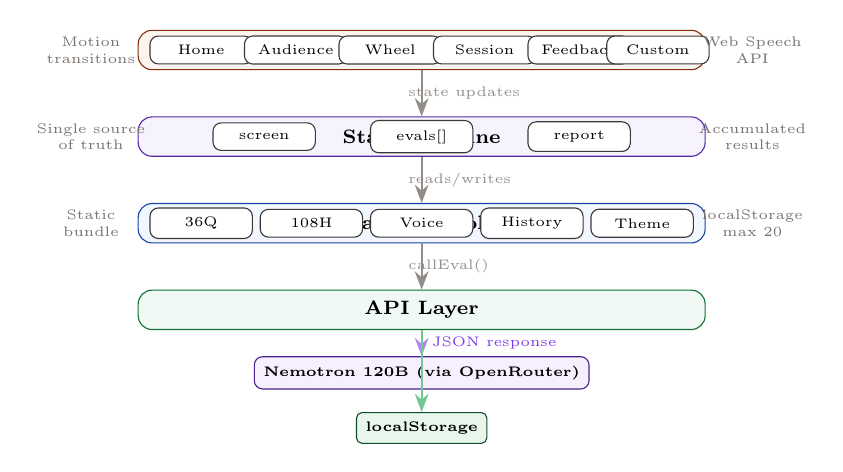
\begin{tikzpicture}[
  >=Stealth,
  layer/.style={draw=accent!70!black, fill=accent!5, rounded corners=5pt, minimum width=7.2cm, minimum height=0.5cm, align=center, font=\scriptsize\bfseries},
  comp/.style={draw=txt2!50!black, fill=white, rounded corners=3pt, minimum width=1.3cm, minimum height=0.35cm, align=center, font=\tiny},
  ext/.style={draw=secondary!60!black, fill=secondary!8, rounded corners=3pt, minimum width=2.4cm, minimum height=0.4cm, align=center, font=\tiny\bfseries},
  arrow/.style={->, thick, color=txt2!80},
  data/.style={font=\tiny, text=txt2, align=center},
]

\node[layer, fill=accent!6] (pres) at (0, 3.6) {Presentation Layer};
\node[layer, fill=secondary!6, draw=secondary!70!black] (state) at (0, 2.5) {State Machine};
\node[layer, fill=bluea!6, draw=bluea!70!black] (dataL) at (0, 1.4) {Data \& Hooks};
\node[layer, fill=success!6, draw=success!70!black] (api) at (0, 0.3) {API Layer};

\node[comp] (s1) at (-2.8, 3.6) {Home};
\node[comp] (s2) at (-1.6, 3.6) {Audience};
\node[comp] (s3) at (-0.4, 3.6) {Wheel};
\node[comp] (s4) at (0.8, 3.6) {Session};
\node[comp] (s5) at (2.0, 3.6) {Feedback};
\node[comp] (s6) at (3.0, 3.6) {Custom};

\node[comp] (sv) at (-2.0, 2.5) {screen};
\node[comp] (ev) at (0, 2.5) {evals[]};
\node[comp] (rp) at (2.0, 2.5) {report};

\node[comp] (q) at (-2.8, 1.4) {36Q};
\node[comp] (h) at (-1.4, 1.4) {108H};
\node[comp] (v) at (0, 1.4) {Voice};
\node[comp] (hs) at (1.4, 1.4) {History};
\node[comp] (th) at (2.8, 1.4) {Theme};

\node[ext] (llm) at (0, -0.5) {Nemotron 120B (via OpenRouter)};

\node[data, align=center] at (-4.2, 3.6) {Motion\\transitions};
\node[data, align=center] at (4.2, 3.6) {Web Speech\\API};
\node[data, align=center] at (-4.2, 2.5) {Single source\\of truth};
\node[data, align=center] at (4.2, 2.5) {Accumulated\\results};
\node[data, align=center] at (-4.2, 1.4) {Static\\bundle};
\node[data, align=center] at (4.2, 1.4) {localStorage\\max 20};

\draw[arrow] (pres.south) -- node[right, font=\tiny, xshift=-0.3cm] {state updates} (state.north);
\draw[arrow] (state.south) -- node[right, font=\tiny, xshift=-0.3cm] {reads/writes} (dataL.north);
\draw[arrow] (dataL.south) -- node[right, font=\tiny, xshift=-0.3cm] {callEval()} (api.north);
\draw[arrow, dashed, color=secondary!60] (api.south) -- node[right, font=\tiny, color=secondary] {JSON response} (llm.north);

\node[draw=success!50!black, fill=success!10, rounded corners=2pt, minimum width=1.2cm, minimum height=0.3cm, font=\tiny\bfseries] (ls) at (0, -1.2) {localStorage};
\draw[arrow, color=success!60] (api.south) -- ++(0,-0.2) -| (ls.north);

\end{tikzpicture}
\caption{Four-layer architecture of TeachLoop with component inventory and data flow annotations.}
\label{fig:arch}
\end{figure}

The Presentation layer contains seven screen components (Home, Audience, Wheel, Session, Feedback, CustomMode, CustomReview) with Motion-powered page transitions. The State Machine layer manages all application state via \texttt{useState} hooks in the root \texttt{AppInner} component---there is no client-side router; a \texttt{screen} state variable controls which screen is rendered. The Data \& Hooks layer provides static question banks, progressive hints, voice input via the Web Speech API, and localStorage session persistence. The API layer consists of a single Next.js API route that proxies evaluation requests to OpenRouter.

\subsection{Screen State Machine}

The application operates as a finite state machine with 8 screens (Fig.~\ref{fig:state}). The \texttt{screen} state variable is the single source of truth for navigation state. There is no URL-based routing---the browser URL remains \texttt{/} throughout the entire session.

\begin{figure}[!t]
\centering
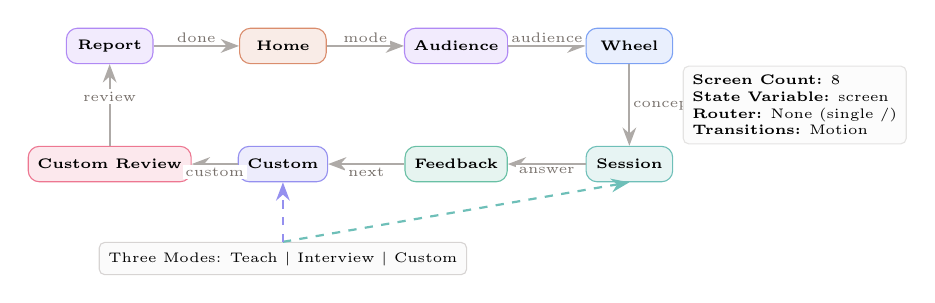
\begin{tikzpicture}[
  >=Stealth,
  scrn/.style={rectangle, rounded corners=4pt, minimum width=1.1cm, minimum height=0.45cm, text centered, font=\tiny\bfseries},
  arr/.style={->, thick, color=txt2!60},
  lbl/.style={font=\tiny, text=txt2, fill=white, inner sep=1pt},
]

\node[scrn, draw=accent!60, fill=accent!10] (home) at (0, 3) {Home};
\node[scrn, draw=secondary!60, fill=secondary!10] (audience) at (2.2, 3) {Audience};
\node[scrn, draw=bluea!60, fill=bluea!10] (wheel) at (4.4, 3) {Wheel};
\node[scrn, draw=teal!60, fill=teal!10] (session) at (4.4, 1.5) {Session};
\node[scrn, draw=emerald!60, fill=emerald!10] (feedback) at (2.2, 1.5) {Feedback};
\node[scrn, draw=indigo!60, fill=indigo!10] (custom) at (0, 1.5) {Custom};
\node[scrn, draw=rose!60, fill=rose!10, align=center] (customreview) at (-2.2, 1.5) {Custom Review};
\node[scrn, draw=violet!60, fill=violet!10] (report) at (-2.2, 3) {Report};

\node[draw=txt2!30, fill=txt2!3, rounded corners=2pt, font=\tiny, align=center] (modes) at (0, 0.3) {Three Modes: Teach $\mid$ Interview $\mid$ Custom};

\draw[arr] (home) -- node[lbl, above] {mode} (audience);
\draw[arr] (audience) -- node[lbl, above] {audience} (wheel);
\draw[arr] (wheel) -- node[lbl, right] {concept} (session);
\draw[arr] (session) -- node[lbl, below] {answer} (feedback);
\draw[arr] (feedback) -- node[lbl, below] {next} (custom);
\draw[arr] (custom) -- node[lbl, below] {custom} (customreview);
\draw[arr] (customreview) -- node[lbl, above] {review} (report);
\draw[arr] (report) -- node[lbl, above] {done} (home);

\draw[arr, dashed, color=teal!60] (modes.north) -- (session.south);
\draw[arr, dashed, color=indigo!60] (modes.north) -- (custom.south);

\node[draw=txt2!20, fill=txt2!2, rounded corners=2pt, font=\tiny, align=left] at (6.5, 2.25) {
  \textbf{Screen Count:} 8\\
  \textbf{State Variable:} screen\\
  \textbf{Router:} None (single /)\\
  \textbf{Transitions:} Motion
};

\end{tikzpicture}
\caption{Screen state machine with 8 screens. The \texttt{screen} state variable controls navigation without URL routing.}
\label{fig:state}
\end{figure}

The root component maintains 18 state variables that collectively encode the full application state. Table~\ref{tab:state} enumerates the key state variables and their roles.

\begin{table}[!t]
\centering
\caption{Key Application State Variables}
\label{tab:state}
\begin{tabularx}{\columnwidth}{lX}
\toprule
\textbf{Variable} & \textbf{Role} \\
\midrule
\texttt{screen} & Current screen (8 values) \\
\texttt{mode} & teach / interview / custom \\
\texttt{qs} & Question array for session \\
\texttt{idx} & Current question index \\
\texttt{ans} & Current answer text \\
\texttt{evals} & Accumulated evaluations \\
\texttt{report} & Session summary \\
\texttt{wheelSpin} & Animation state \\
\texttt{wasVoiceUsed} & Microphone flag \\
\texttt{hintLevel} & 0 / 1 / 2 / 3 \\
\bottomrule
\end{tabularx}
\end{table}

\subsection{AI Evaluation Pipeline}

Each user answer is evaluated by an LLM through a structured pipeline (Fig.~\ref{fig:eval}). The pipeline implements five validation stages before reaching the AI model.

\begin{figure}[!t]
\centering
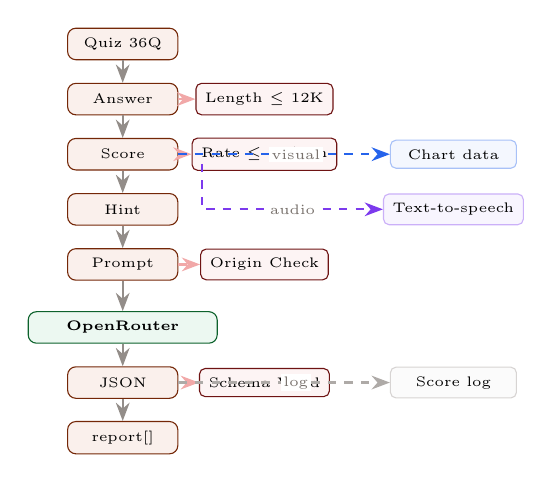
\begin{tikzpicture}[
  >=Stealth,
  evalStep/.style={draw=accent!60!black, fill=accent!8, rounded corners=3pt, minimum width=1.4cm, minimum height=0.4cm, align=center, font=\tiny},
  api/.style={draw=success!60!black, fill=success!8, rounded corners=3pt, minimum width=2.4cm, minimum height=0.4cm, align=center, font=\tiny\bfseries},
  arr/.style={->, thick, color=txt2!80},
  elbl/.style={font=\tiny, text=txt2, fill=white, inner sep=1pt, pos=0.55},
  guard/.style={draw=err!50!black, fill=err!5, rounded corners=2pt, minimum width=1.0cm, minimum height=0.3cm, align=center, font=\tiny},
]

\node[evalStep] (q) at (0, 3.2) {Quiz 36Q};
\node[evalStep] (a) at (0, 2.5) {Answer};
\node[guard] (g1) at (1.8, 2.5) {Length $\leq$ 12K};
\node[evalStep] (s) at (0, 1.8) {Score};
\node[guard] (g2) at (1.8, 1.8) {Rate $\leq$ 30/min};
\node[evalStep] (h) at (0, 1.1) {Hint};
\node[evalStep] (p) at (0, 0.4) {Prompt};
\node[guard] (g3) at (1.8, 0.4) {Origin Check};
\node[api] (api) at (0, -0.4) {OpenRouter};
\node[evalStep] (r) at (0, -1.1) {JSON};
\node[guard] (g4) at (1.8, -1.1) {Schema Valid};
\node[evalStep] (re) at (0, -1.8) {report[]};

\node[draw=secondary!40, fill=secondary!5, rounded corners=2pt, minimum width=1.6cm, minimum height=0.3cm, font=\tiny] (t) at (4.2, 1.1) {Text-to-speech};
\node[draw=bluea!40, fill=bluea!5, rounded corners=2pt, minimum width=1.6cm, minimum height=0.3cm, font=\tiny] (v) at (4.2, 1.8) {Chart data};
\node[draw=txt2!30, fill=txt2!3, rounded corners=2pt, minimum width=1.6cm, minimum height=0.3cm, font=\tiny] (l) at (4.2, -1.1) {Score log};

\draw[arr] (q.south) -- (a.north);
\draw[arr] (a.south) -- (s.north);
\draw[arr] (s.south) -- (h.north);
\draw[arr] (h.south) -- (p.north);
\draw[arr] (p.south) -- (api.north);
\draw[arr] (api.south) -- (r.north);
\draw[arr] (r.south) -- (re.north);

\draw[arr, dashed, color=err!40] (a.east) -- (g1.west);
\draw[arr, dashed, color=err!40] (s.east) -- (g2.west);
\draw[arr, dashed, color=err!40] (p.east) -- (g3.west);
\draw[arr, dashed, color=err!40] (r.east) -- (g4.west);

\draw[arr, dashed, color=secondary] (s.east) -- ++(0.3,0) |- node[elbl, near end] {audio} (t.west);
\draw[arr, dashed, color=bluea] (s.east) -- ++(0.3,0) |- node[elbl, near end] {visual} (v.west);
\draw[arr, dashed, color=txt2!60] (r.east) -- ++(0.3,0) |- node[elbl, near end] {log} (l.west);

\end{tikzpicture}
\caption{Evaluation pipeline with four validation guards (right). Dashed lines indicate data consumers.}
\label{fig:eval}
\end{figure}

The prompt construction stage builds a mode-specific evaluation prompt (Fig.~\ref{fig:prompt}). Teaching mode evaluates: clarity, analogies, vocabulary fit, confidence, and structure. Interview mode evaluates: clarity, depth, structure, confidence, and examples. Each dimension is scored 1--10.

\begin{figure}[!t]
\centering
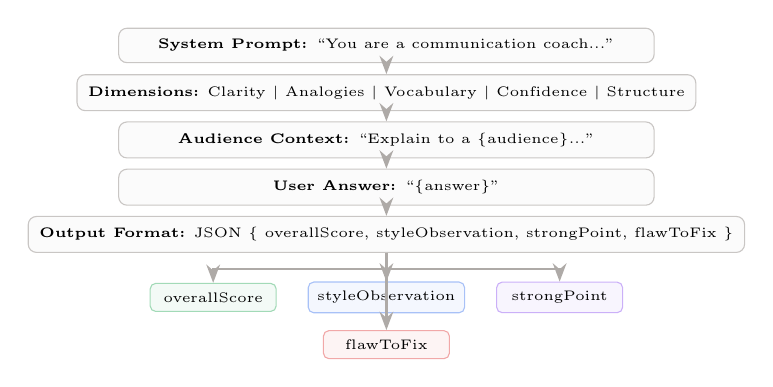
\begin{tikzpicture}[
  >=Stealth,
  block/.style={draw=txt2!40, fill=txt2!3, rounded corners=3pt, minimum width=6.8cm, minimum height=0.35cm, align=left, font=\tiny, inner sep=4pt},
  field/.style={draw=accent!40, fill=accent!5, rounded corners=2pt, minimum width=1.6cm, minimum height=0.3cm, align=center, font=\tiny},
  arr/.style={->, thick, color=txt2!60},
]

\node[block] (header) at (0, 2.8) {\textbf{System Prompt:} ``You are a communication coach...''};
\node[block] (dims) at (0, 2.2) {\textbf{Dimensions:} Clarity $\mid$ Analogies $\mid$ Vocabulary $\mid$ Confidence $\mid$ Structure};
\node[block] (audience) at (0, 1.6) {\textbf{Audience Context:} ``Explain to a \{audience\}...''};
\node[block] (answer) at (0, 1.0) {\textbf{User Answer:} ``\{answer\}''};
\node[block] (format) at (0, 0.4) {\textbf{Output Format:} JSON \{ overallScore, styleObservation, strongPoint, flawToFix \}};

\node[field, fill=success!5, draw=success!40] (os) at (-2.2, -0.4) {overallScore};
\node[field, fill=bluea!5, draw=bluea!40] (so) at (0, -0.4) {styleObservation};
\node[field, fill=secondary!5, draw=secondary!40] (sp) at (2.2, -0.4) {strongPoint};
\node[field, fill=err!5, draw=err!40] (ff) at (0, -1.0) {flawToFix};

\draw[arr] (header.south) -- (dims.north);
\draw[arr] (dims.south) -- (audience.north);
\draw[arr] (audience.south) -- (answer.north);
\draw[arr] (answer.south) -- (format.north);
\draw[arr] (format.south) -- ++(0,-0.2) -| (os.north);
\draw[arr] (format.south) -- ++(0,-0.2) -| (so.north);
\draw[arr] (format.south) -- ++(0,-0.2) -| (sp.north);
\draw[arr] (format.south) -- ++(0,-0.2) -| (ff.north);

\end{tikzpicture}
\caption{AI evaluation prompt structure with system instructions, dimension scoring, and JSON output schema.}
\label{fig:prompt}
\end{figure}

Input validation caps prompt length at 12,000 characters. Rate limiting enforces 30 requests per minute per IP address using an in-memory store. The API call uses a 15-second timeout via \texttt{AbortController} with exponential backoff retry (2 attempts). JSON extraction includes fallback parsing for malformed responses. Schema validation ensures the response matches the expected shape before returning to the client.

After all questions in a session are evaluated, a session report is generated by aggregating individual evaluations into a communication style analysis, recurring strength, recurring flaw, and a weekly practice tip. This report is saved to localStorage as part of the session history.

\subsection{Progressive Hint System}

Each of the 36 static concepts offers three hint levels following scaffolding theory~\cite{vanlehn} (Fig.~\ref{fig:hints}):

\begin{figure}[!t]
\centering
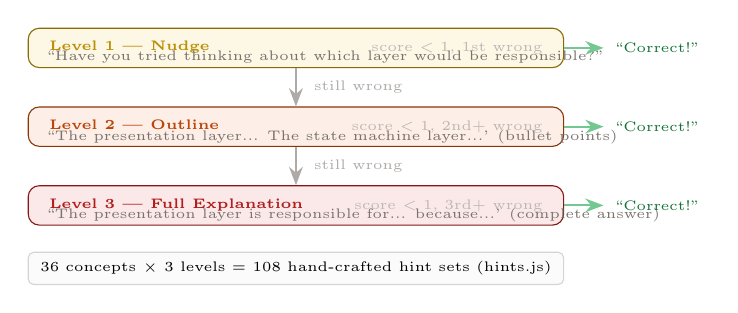
\begin{tikzpicture}[
  >=Stealth,
  lvl/.style={draw=#1!60!black, fill=#1!10, rounded corners=4pt, minimum width=6.8cm, minimum height=0.5cm, align=left, font=\tiny},
  ex/.style={font=\tiny, text=txt2, align=left, inner sep=2pt},
  arr/.style={->, thick, color=txt2!60},
]

\node[lvl=l1, minimum width=6.8cm] (L1) at (0, 3.0) {};
\node[font=\tiny\bfseries, text=l1!80!black, anchor=north west] at ([xshift=0.15cm, yshift=-0.05cm]L1.north west) {Level 1 --- Nudge};
\node[ex, anchor=north west] at ([xshift=0.15cm, yshift=-0.22cm]L1.north west) {``Have you tried thinking about which layer would be responsible?''};
\node[font=\tiny, text=txt2!50, anchor=south east] at ([xshift=-0.15cm, yshift=0.05cm]L1.south east) {score $< 1$, 1st wrong};

\node[lvl=l2, minimum width=6.8cm] (L2) at (0, 2.0) {};
\node[font=\tiny\bfseries, text=l2!80!black, anchor=north west] at ([xshift=0.15cm, yshift=-0.05cm]L2.north west) {Level 2 --- Outline};
\node[ex, anchor=north west] at ([xshift=0.15cm, yshift=-0.22cm]L2.north west) {``The presentation layer... The state machine layer...' (bullet points)};
\node[font=\tiny, text=txt2!50, anchor=south east] at ([xshift=-0.15cm, yshift=0.05cm]L2.south east) {score $< 1$, 2nd+ wrong};

\node[lvl=l3, minimum width=6.8cm] (L3) at (0, 1.0) {};
\node[font=\tiny\bfseries, text=l3!80!black, anchor=north west] at ([xshift=0.15cm, yshift=-0.05cm]L3.north west) {Level 3 --- Full Explanation};
\node[ex, anchor=north west] at ([xshift=0.15cm, yshift=-0.22cm]L3.north west) {``The presentation layer is responsible for... because...' (complete answer)};
\node[font=\tiny, text=txt2!50, anchor=south east] at ([xshift=-0.15cm, yshift=0.05cm]L3.south east) {score $< 1$, 3rd+ wrong};

\draw[arr] (L1.south) -- node[right, font=\tiny, xshift=0.1cm] {still wrong} (L2.north);
\draw[arr] (L2.south) -- node[right, font=\tiny, xshift=0.1cm] {still wrong} (L3.north);

\draw[arr, color=success!60] (L1.east) -- ++(0.5,0) node[right, font=\tiny, text=success!70!black] {``Correct!''};
\draw[arr, color=success!60] (L2.east) -- ++(0.5,0) node[right, font=\tiny, text=success!70!black] {``Correct!''};
\draw[arr, color=success!60] (L3.east) -- ++(0.5,0) node[right, font=\tiny, text=success!70!black] {``Correct!''};

\node[draw=txt2!30, fill=txt2!3, rounded corners=2pt, minimum width=6.8cm, minimum height=0.3cm, font=\tiny, align=center] at (0, 0.2) {36 concepts $\times$ 3 levels = 108 hand-crafted hint sets (hints.js)};

\end{tikzpicture}
\caption{Three-level progressive hint system. Each level adds cognitive scaffolding.}
\label{fig:hints}
\end{figure}

\begin{enumerate}[leftmargin=*, label=\textbf{L\arabic*:}]
  \item \textbf{Nudge:} A gentle directional prompt that points toward the answer without revealing it. Example for ``Attention Mechanism'': ``Focus on the core idea of weighing how much each input word matters to every other word.''
  \item \textbf{Concept Outline:} A structured scaffold providing key concepts and terminology. Example: ``Attention lets each token look at all other tokens and decide which ones are most relevant. Explain query, key, value vectors and the softmax weighting.''
  \item \textbf{Full Explanation:} A comprehensive reference covering what a strong answer should include. Example: ``In `Attention Is All You Need', each token is projected into Q, K, V. Attention scores = softmax(QK$^T$/$\sqrt{d}$)V. Multi-head attention runs this in parallel.''
\end{enumerate}

The content database covers 20 AI/ML teaching concepts (from Backpropagation to Mixture of Experts) and 16 system design/SWE interview questions (from URL shortening to consensus algorithms). Each hint set is hand-curated to ensure technical accuracy and pedagogical progression.

\subsection{Voice Input Pipeline}

The \texttt{useVoice} hook captures speech via the Web Speech API and applies automatic post-processing (Fig.~\ref{fig:voice}). Filler words (``um,'' ``uh,'' ``like,'' ``you know,'' ``I mean,'' ``basically,'' ``literally,'' ``right'') are removed. Consecutive duplicate words are collapsed. Punctuation is normalized. A \texttt{wasVoiceUsed} flag annotates the evaluation prompt to excuse transcription artifacts: ``Grade the ideas and communication, not the transcription quality.''

\begin{figure}[!t]
\centering
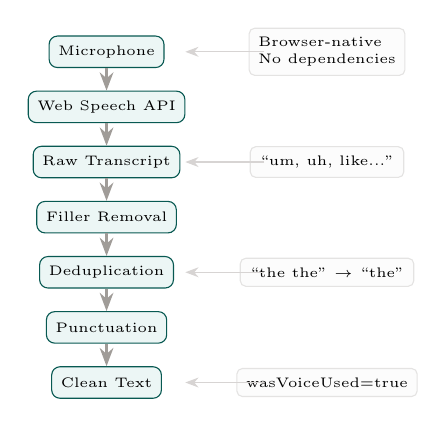
\begin{tikzpicture}[
  >=Stealth,
  vstep/.style={draw=teal!60!black, fill=teal!8, rounded corners=3pt, minimum width=1.3cm, minimum height=0.4cm, align=center, font=\tiny},
  arr/.style={->, thick, color=txt2!70},
]

\node[vstep] (mic) at (0, 2.5) {Microphone};
\node[vstep] (api) at (0, 1.8) {Web Speech API};
\node[vstep] (raw) at (0, 1.1) {Raw Transcript};
\node[vstep] (filler) at (0, 0.4) {Filler Removal};
\node[vstep] (dedup) at (0, -0.3) {Deduplication};
\node[vstep] (punct) at (0, -1.0) {Punctuation};
\node[vstep] (clean) at (0, -1.7) {Clean Text};

\node[draw=txt2!20, fill=txt2!2, rounded corners=2pt, font=\tiny, align=left] at (2.8, 2.5) {Browser-native \\ No dependencies};
\node[draw=txt2!20, fill=txt2!2, rounded corners=2pt, font=\tiny, align=left] at (2.8, 1.1) {``um, uh, like...''};
\node[draw=txt2!20, fill=txt2!2, rounded corners=2pt, font=\tiny, align=left] at (2.8, -0.3) {``the the'' $\to$ ``the''};
\node[draw=txt2!20, fill=txt2!2, rounded corners=2pt, font=\tiny, align=left] at (2.8, -1.7) {wasVoiceUsed=true};

\draw[arr] (mic) -- (api);
\draw[arr] (api) -- (raw);
\draw[arr] (raw) -- (filler);
\draw[arr] (filler) -- (dedup);
\draw[arr] (dedup) -- (punct);
\draw[arr] (punct) -- (clean);

\draw[->, thin, color=txt2!30] (2.0, 2.5) -- (1.0, 2.5);
\draw[->, thin, color=txt2!30] (2.0, 1.1) -- (1.0, 1.1);
\draw[->, thin, color=txt2!30] (2.0, -0.3) -- (1.0, -0.3);
\draw[->, thin, color=txt2!30] (2.0, -1.7) -- (1.0, -1.7);

\end{tikzpicture}
\caption{Voice input pipeline with automatic post-processing stages.}
\label{fig:voice}
\end{figure}

\subsection{Data Architecture}

All data is client-side (Fig.~\ref{fig:data}). Static content (36 questions, 108 hint sets, 5 audience definitions) is bundled as JavaScript modules. Session history (date, mode, audience, overall score, per-question scores) persists in localStorage with a 20-session cap. Theme preference and onboarding dismissal state also persist. There is no server-side database, no user authentication, and no cross-device synchronization.

\begin{figure}[!t]
\centering
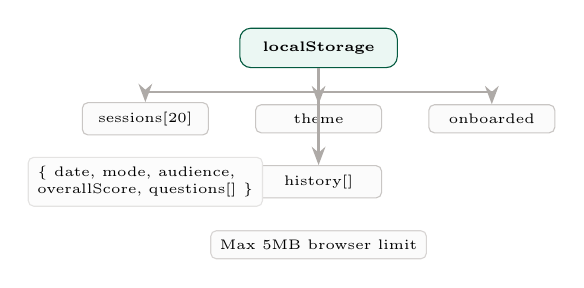
\begin{tikzpicture}[
  >=Stealth,
  store/.style={draw=emerald!60!black, fill=emerald!8, rounded corners=4pt, minimum width=2.0cm, minimum height=0.5cm, align=center, font=\tiny\bfseries},
  item/.style={draw=txt2!40, fill=txt2!3, rounded corners=2pt, minimum width=1.6cm, minimum height=0.3cm, align=center, font=\tiny},
  arr/.style={->, thick, color=txt2!60},
]

\node[store] (ls) at (0, 2.5) {localStorage};

\node[item] (sess) at (-2.2, 1.6) {sessions[20]};
\node[item] (theme) at (0, 1.6) {theme};
\node[item] (onboard) at (2.2, 1.6) {onboarded};
\node[item] (hist) at (0, 0.8) {history[]};

\node[draw=txt2!20, fill=txt2!2, rounded corners=2pt, font=\tiny, align=left] at (-2.2, 0.8) {
  \{ date, mode, audience,\\
  overallScore, questions[] \}
};

\draw[arr] (ls.south) -- ++(0,-0.3) -| (sess.north);
\draw[arr] (ls.south) -- (theme.north);
\draw[arr] (ls.south) -- ++(0,-0.3) -| (onboard.north);
\draw[arr] (ls.south) -- (hist.north);

\node[draw=txt2!30, fill=txt2!3, rounded corners=2pt, font=\tiny, align=center] at (0, 0.0) {Max 5MB browser limit};

\end{tikzpicture}
\caption{localStorage data architecture with schema and size constraints.}
\label{fig:data}
\end{figure}

% ══════════════════════════════════════════════════════════
\section{Design System}
\label{sec:design-system}

\subsection{Typography and Spacing}

The typography follows a Perfect Fourth (1.333) modular scale with 10 defined steps from 0.6875rem (2xs) to 3.375rem (5xl). The primary typeface is Geist, a variable font optimized for screen reading. Spacing uses a 4pt base with 16 defined steps from 0.25rem to 8rem. Border radii range from 0.25rem (xs) to 9999px (full). Easing curves include quart, expo, spring, and in-out variants. A z-index scale from 0 (base) to 500 (toast) prevents stacking conflicts.

\begin{figure}[!t]
\centering
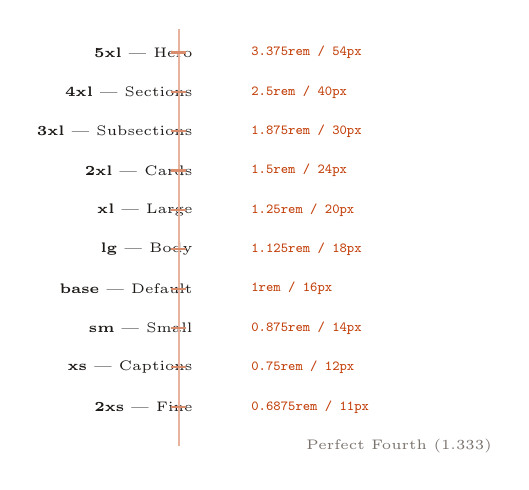
\begin{tikzpicture}[
  >=Stealth,
  type/.style={font=\tiny, text=txt, align=left},
  size/.style={font=\tiny\ttfamily, text=accent},
]

\node[type, anchor=east] at (0, 3.5) {\textbf{5xl} --- Hero};
\node[size, anchor=west] at (0.5, 3.5) {3.375rem / 54px};

\node[type, anchor=east] at (0, 3.0) {\textbf{4xl} --- Sections};
\node[size, anchor=west] at (0.5, 3.0) {2.5rem / 40px};

\node[type, anchor=east] at (0, 2.5) {\textbf{3xl} --- Subsections};
\node[size, anchor=west] at (0.5, 2.5) {1.875rem / 30px};

\node[type, anchor=east] at (0, 2.0) {\textbf{2xl} --- Cards};
\node[size, anchor=west] at (0.5, 2.0) {1.5rem / 24px};

\node[type, anchor=east] at (0, 1.5) {\textbf{xl} --- Large};
\node[size, anchor=west] at (0.5, 1.5) {1.25rem / 20px};

\node[type, anchor=east] at (0, 1.0) {\textbf{lg} --- Body};
\node[size, anchor=west] at (0.5, 1.0) {1.125rem / 18px};

\node[type, anchor=east] at (0, 0.5) {\textbf{base} --- Default};
\node[size, anchor=west] at (0.5, 0.5) {1rem / 16px};

\node[type, anchor=east] at (0, 0.0) {\textbf{sm} --- Small};
\node[size, anchor=west] at (0.5, 0.0) {0.875rem / 14px};

\node[type, anchor=east] at (0, -0.5) {\textbf{xs} --- Captions};
\node[size, anchor=west] at (0.5, -0.5) {0.75rem / 12px};

\node[type, anchor=east] at (0, -1.0) {\textbf{2xs} --- Fine};
\node[size, anchor=west] at (0.5, -1.0) {0.6875rem / 11px};

\draw[thick, color=accent!40] (-0.3, -1.5) -- (-0.3, 3.8);
\foreach \y in {3.5, 3.0, 2.5, 2.0, 1.5, 1.0, 0.5, 0.0, -0.5, -1.0} {
  \draw[thick, color=accent!60] (-0.4, \y) -- (-0.2, \y);
}

\node[font=\tiny, text=txt2] at (2.5, -1.5) {Perfect Fourth (1.333)};

\end{tikzpicture}
\caption{Typography scale with Perfect Fourth modular ratio.}
\label{fig:typography}
\end{figure}

\subsection{Theme System}

Three themes are implemented via CSS custom properties, each defining 40+ variables for colors, shadows, grain texture, glass effects, and wheel segment colors (Table~\ref{tab:themes}).

\begin{table}[!t]
\centering
\caption{Theme Variants with Accent Colors}
\label{tab:themes}
\begin{tabular}{lll}
\toprule
\textbf{Theme} & \textbf{Accent} & \textbf{Background} \\
\midrule
Sunrise Studio & Burnt Orange \#C2410C & Warm cream \#FBF9F6 \\
Chalkboard & Yellow \#FACC15 & Dark zinc \#18181B \\
Blue Hour & Blue \#2563EB & Cool slate \#F8FAFC \\
\bottomrule
\end{tabular}
\end{table}

Theme selection persists in localStorage and is applied via the \texttt{data-theme} attribute on the document root. An inline script in the root layout runs before React hydration to prevent flash-of-unstyled-theme (FOUC). The \texttt{ThemeProvider} context exposes the current theme and a switcher component (three colored dots with spring-scale animation).

\begin{figure}[!t]
\centering
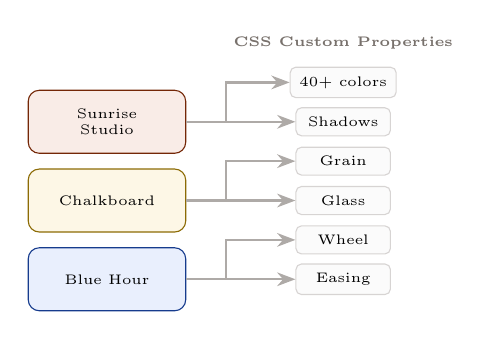
\begin{tikzpicture}[
  >=Stealth,
  thm/.style={draw=#1!60!black, fill=#1!10, rounded corners=4pt, minimum width=2.0cm, minimum height=0.8cm, align=center, font=\tiny},
  prop/.style={draw=txt2!30, fill=txt2!3, rounded corners=2pt, minimum width=1.2cm, minimum height=0.25cm, align=center, font=\tiny},
  arr/.style={->, thick, color=txt2!60},
]

\node[thm=accent, align=center] (sunrise) at (0, 2.0) {Sunrise\\Studio};
\node[thm=l1] (chalk) at (0, 1.0) {Chalkboard};
\node[thm=bluea] (blue) at (0, 0.0) {Blue Hour};

\node[prop] (colors) at (3.0, 2.5) {40+ colors};
\node[prop] (shadows) at (3.0, 2.0) {Shadows};
\node[prop] (grain) at (3.0, 1.5) {Grain};
\node[prop] (glass) at (3.0, 1.0) {Glass};
\node[prop] (wheel) at (3.0, 0.5) {Wheel};
\node[prop] (ease) at (3.0, 0.0) {Easing};

\draw[arr] (sunrise.east) -- ++(0.5,0) |- (colors.west);
\draw[arr] (sunrise.east) -- ++(0.5,0) |- (shadows.west);
\draw[arr] (chalk.east) -- ++(0.5,0) |- (grain.west);
\draw[arr] (chalk.east) -- ++(0.5,0) |- (glass.west);
\draw[arr] (blue.east) -- ++(0.5,0) |- (wheel.west);
\draw[arr] (blue.east) -- ++(0.5,0) |- (ease.west);

\node[font=\tiny\bfseries, text=txt2] at (3.0, 3.0) {CSS Custom Properties};

\end{tikzpicture}
\caption{Theme architecture showing CSS custom property categories per theme.}
\label{fig:themes}
\end{figure}

\subsection{Visual Effects}

The design system employs seven layered visual effects:

\begin{enumerate}[leftmargin=*, label=(\arabic*)]
  \item \textbf{Grain Texture:} An SVG noise overlay at 2--4\% opacity is applied via a \texttt{::after} pseudo-element on the body, adding tactile warmth without impacting readability.
  \item \textbf{Glassmorphism:} The navigation bar uses \texttt{backdrop-filter: blur(16px)} with a semi-transparent background, creating a depth hierarchy between the nav and page content.
  \item \textbf{ScoreRing:} An SVG circle with animated \texttt{stroke-dashoffset} represents scores. Color coding: green for scores $\geq$8, accent for 5--7, red for $<$5. Configurable size and animation delay.
  \item \textbf{Sparkline Charts:} SVG polylines render score trends across past sessions. Auto-scales to min/max range. Up to 5 sessions are shown on the home screen.
  \item \textbf{Wheel Animation:} A CSS conic-gradient wheel with segment labels spins using quadratic easing (3--5 extra rotations). A glow effect activates during spin. Progress dots with connecting lines track completed questions.
  \item \textbf{Page Transitions:} \texttt{AnimatePresence} with 250ms opacity fade between all screens.
  \item \textbf{Staggered Entrances:} Audience list items animate in with 50ms stagger delay for a polished reveal effect.
\end{enumerate}

\begin{figure}[!t]
\centering
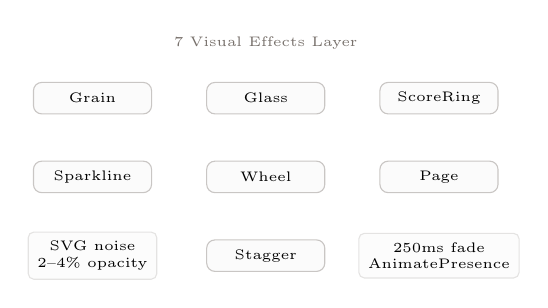
\begin{tikzpicture}[
  >=Stealth,
  effect/.style={draw=txt2!40, fill=txt2!3, rounded corners=3pt, minimum width=1.5cm, minimum height=0.4cm, align=center, font=\tiny},
]

\node[effect] (grain) at (0, 2.5) {Grain};
\node[effect] (glass) at (2.2, 2.5) {Glass};
\node[effect] (ring) at (4.4, 2.5) {ScoreRing};
\node[effect] (spark) at (0, 1.5) {Sparkline};
\node[effect] (wheel) at (2.2, 1.5) {Wheel};
\node[effect] (page) at (4.4, 1.5) {Page};
\node[effect] (stagger) at (2.2, 0.5) {Stagger};

\node[draw=txt2!20, fill=txt2!2, rounded corners=2pt, font=\tiny, align=center] at (0, 0.5) {SVG noise \\ 2--4\% opacity};
\node[draw=txt2!20, fill=txt2!2, rounded corners=2pt, font=\tiny, align=center] at (4.4, 0.5) {250ms fade \\ AnimatePresence};

\node[font=\tiny, text=txt2] at (2.2, 3.2) {7 Visual Effects Layer};

\end{tikzpicture}
\caption{Seven visual effects implemented in the design system.}
\label{fig:effects}
\end{figure}

% ══════════════════════════════════════════════════════════
\section{Implementation}
\label{sec:implementation}

\subsection{Technology Stack}

Table~\ref{tab:stack} summarizes the technology stack and the rationale for each choice.

\begin{table}[!t]
\centering
\caption{Technology Stack}
\label{tab:stack}
\begin{tabularx}{\columnwidth}{lX}
\toprule
\textbf{Component} & \textbf{Technology \& Rationale} \\
\midrule
Framework & Next.js 15.3.3 (App Router, API routes, React Server Components) \\
UI & React 19.1.0 (concurrent features, Suspense for code splitting) \\
Animation & Motion 12.42.0 (spring physics, AnimatePresence) \\
Typography & Geist 1.7.2 (variable font, screen-optimized) \\
Icons & Phosphor Icons 2.1.10 (duotone weight, consistent language) \\
AI Backend & OpenRouter / NVIDIA Nemotron 120B (free tier, JSON mode) \\
Speech & Web Speech API (native browser, no dependencies) \\
Storage & localStorage (max 20 sessions, JSON serialization) \\
Deployment & Vercel (edge functions, zero-config Next.js) \\
\bottomrule
\end{tabularx}
\end{table}

\subsection{Component Hierarchy}

The React component hierarchy follows a flat structure with the root \texttt{AppInner} component managing all state (Fig.~\ref{fig:components}).

\begin{figure}[!t]
\centering
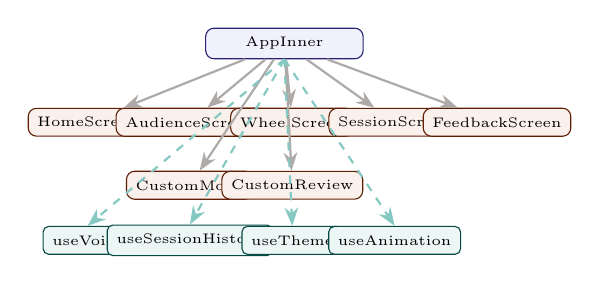
\begin{tikzpicture}[
  >=Stealth,
  comp/.style={draw=indigo!50!black, fill=indigo!8, rounded corners=3pt, minimum width=1.4cm, minimum height=0.35cm, align=center, font=\tiny},
  scrn/.style={draw=accent!50!black, fill=accent!8, rounded corners=3pt, minimum width=1.2cm, minimum height=0.3cm, align=center, font=\tiny},
  hook/.style={draw=teal!50!black, fill=teal!8, rounded corners=2pt, minimum width=1.0cm, minimum height=0.25cm, align=center, font=\tiny},
  arr/.style={->, thick, color=txt2!60},
]

\node[comp, minimum width=2.0cm] (root) at (0, 3) {AppInner};

\node[scrn] (home) at (-2.5, 2) {HomeScreen};
\node[scrn] (aud) at (-1.2, 2) {AudienceScreen};
\node[scrn] (wheel) at (0.1, 2) {WheelScreen};
\node[scrn] (sess) at (1.4, 2) {SessionScreen};
\node[scrn] (fb) at (2.7, 2) {FeedbackScreen};
\node[scrn] (custom) at (-1.2, 1.2) {CustomMode};
\node[scrn] (crev) at (0.1, 1.2) {CustomReview};

\node[hook] (voice) at (-2.5, 0.5) {useVoice};
\node[hook] (hist) at (-1.2, 0.5) {useSessionHistory};
\node[hook] (theme) at (0.1, 0.5) {useTheme};
\node[hook] (anim) at (1.4, 0.5) {useAnimation};

\draw[arr] (root) -- (home);
\draw[arr] (root) -- (aud);
\draw[arr] (root) -- (wheel);
\draw[arr] (root) -- (sess);
\draw[arr] (root) -- (fb);
\draw[arr] (root) -- (custom);
\draw[arr] (root) -- (crev);

\draw[arr, dashed, color=teal!50] (root.south) -- (voice.north);
\draw[arr, dashed, color=teal!50] (root.south) -- (hist.north);
\draw[arr, dashed, color=teal!50] (root.south) -- (theme.north);
\draw[arr, dashed, color=teal!50] (root.south) -- (anim.north);

\end{tikzpicture}
\caption{React component hierarchy showing screen components and custom hooks.}
\label{fig:components}
\end{figure}

\subsection{Code Splitting and Dynamic Imports}

Heavy screen components (AudienceScreen, WheelScreen, SessionScreen, FeedbackScreen) use Next.js \texttt{dynamic()} imports with no loading placeholder. The app shell (HomeScreen, CustomModeScreen) loads eagerly. This reduces the initial bundle from the full application to just the entry screen and shared utilities.

\subsection{Error Handling}

A class-based \texttt{ErrorBoundary} component wraps the entire application, catching React rendering errors and providing a recovery UI with a ``Try again'' button (Fig.~\ref{fig:error}). API errors are caught at the call site and displayed in contextual error banners with retry options. The session report generation has independent error handling---if report generation fails, users can still view their individual answers.

\begin{figure}[!t]
\centering
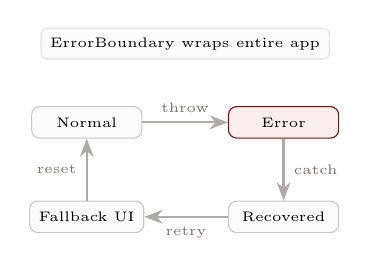
\begin{tikzpicture}[
  >=Stealth,
  state/.style={draw=txt2!40, fill=txt2!3, rounded corners=3pt, minimum width=1.4cm, minimum height=0.4cm, align=center, font=\tiny},
  err/.style={draw=err!50!black, fill=err!8, rounded corners=3pt, minimum width=1.4cm, minimum height=0.4cm, align=center, font=\tiny},
  arr/.style={->, thick, color=txt2!60},
  lbl/.style={font=\tiny, text=txt2},
]

\node[state] (normal) at (0, 2) {Normal};
\node[err] (error) at (2.5, 2) {Error};
\node[state] (recovered) at (2.5, 0.8) {Recovered};
\node[state] (fallback) at (0, 0.8) {Fallback UI};

\draw[arr] (normal) -- node[lbl, above] {throw} (error);
\draw[arr] (error) -- node[lbl, right] {catch} (recovered);
\draw[arr] (recovered) -- node[lbl, below] {retry} (fallback);
\draw[arr] (fallback) -- node[lbl, left] {reset} (normal);

\node[draw=txt2!20, fill=txt2!2, rounded corners=2pt, font=\tiny, align=center] at (1.25, 3) {ErrorBoundary wraps entire app};

\end{tikzpicture}
\caption{Error handling state machine with recovery flow.}
\label{fig:error}
\end{figure}

\subsection{Security}

The API route implements multiple security layers (Fig.~\ref{fig:security}): IP-based rate limiting (30 requests/minute), origin validation against allowed origins, prompt length capping (12,000 characters), 15-second fetch timeout with \texttt{AbortController}, exponential backoff retry (2 attempts maximum), JSON extraction with regex fallback for malformed responses, and response schema validation. Security headers include X-Frame-Options: DENY, X-Content-Type-Options: nosniff, Referrer-Policy, and Permissions-Policy with microphone=self.

\begin{figure}[!t]
\centering
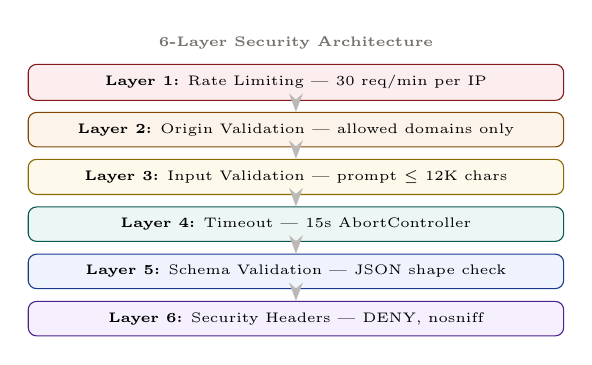
\begin{tikzpicture}[
  >=Stealth,
  layer/.style={draw=#1!60!black, fill=#1!8, rounded corners=3pt, minimum width=6.8cm, minimum height=0.4cm, align=left, font=\tiny, inner sep=4pt},
  arr/.style={->, thick, color=txt2!50},
]

\node[layer=err] (l1) at (0, 2.8) {\textbf{Layer 1:} Rate Limiting --- 30 req/min per IP};
\node[layer=amber] (l2) at (0, 2.2) {\textbf{Layer 2:} Origin Validation --- allowed domains only};
\node[layer=l1] (l3) at (0, 1.6) {\textbf{Layer 3:} Input Validation --- prompt $\leq$ 12K chars};
\node[layer=teal] (l4) at (0, 1.0) {\textbf{Layer 4:} Timeout --- 15s AbortController};
\node[layer=bluea] (l5) at (0, 0.4) {\textbf{Layer 5:} Schema Validation --- JSON shape check};
\node[layer=violet] (l6) at (0, -0.2) {\textbf{Layer 6:} Security Headers --- DENY, nosniff};

\draw[arr] (l1.south) -- (l2.north);
\draw[arr] (l2.south) -- (l3.north);
\draw[arr] (l3.south) -- (l4.north);
\draw[arr] (l4.south) -- (l5.north);
\draw[arr] (l5.south) -- (l6.north);

\node[font=\tiny\bfseries, text=txt2] at (0, 3.3) {6-Layer Security Architecture};

\end{tikzpicture}
\caption{Six-layer security architecture for the API proxy route.}
\label{fig:security}
\end{figure}

\subsection{Accessibility and PWA}

The platform targets WCAG AAA compliance with: a skip link to \texttt{\#main-content}, screen reader text via \texttt{.sr-only} class, \texttt{:focus-visible} outlines with accent color, \texttt{prefers-reduced-motion} media query that disables all animations, semantic HTML with proper heading hierarchy, and full keyboard navigability.

\begin{figure}[!t]
\centering
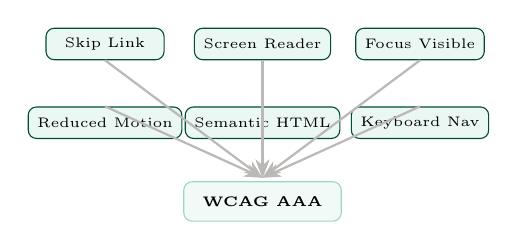
\begin{tikzpicture}[
  >=Stealth,
  feature/.style={draw=emerald!50!black, fill=emerald!8, rounded corners=3pt, minimum width=1.5cm, minimum height=0.4cm, align=center, font=\tiny},
  arr/.style={->, thick, color=txt2!50},
]

\node[feature] (skip) at (-2, 2) {Skip Link};
\node[feature] (sr) at (0, 2) {Screen Reader};
\node[feature] (focus) at (2, 2) {Focus Visible};
\node[feature] (motion) at (-2, 1) {Reduced Motion};
\node[feature] (semantic) at (0, 1) {Semantic HTML};
\node[feature] (keyboard) at (2, 1) {Keyboard Nav};

\node[draw=emerald!40, fill=emerald!5, rounded corners=3pt, minimum width=2.0cm, minimum height=0.5cm, align=center, font=\tiny\bfseries] at (0, 0) {WCAG AAA};

\draw[arr] (skip.south) -- (0, 0.3);
\draw[arr] (sr.south) -- (0, 0.3);
\draw[arr] (focus.south) -- (0, 0.3);
\draw[arr] (motion.north) -- (0, 0.3);
\draw[arr] (semantic.north) -- (0, 0.3);
\draw[arr] (keyboard.north) -- (0, 0.3);

\end{tikzpicture}
\caption{Six accessibility features targeting WCAG AAA compliance.}
\label{fig:accessibility}
\end{figure}

PWA features include a web manifest with app name and theme color, a service worker implementing stale-while-revalidate caching, theme-color meta tag for mobile browser chrome, and a \texttt{beforeunload} handler to prevent accidental navigation during active sessions.

\subsection{API Request/Response Flow}

The complete API flow from client to LLM and back is shown in Fig.~\ref{fig:api}.

\begin{figure}[!t]
\centering
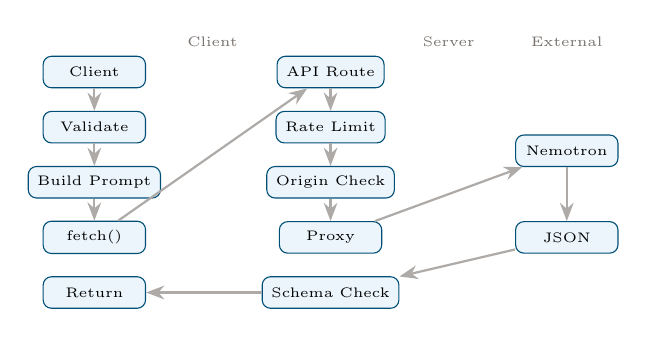
\begin{tikzpicture}[
  >=Stealth,
  astep/.style={draw=sky!60!black, fill=sky!8, rounded corners=3pt, minimum width=1.3cm, minimum height=0.4cm, align=center, font=\tiny},
  arr/.style={->, thick, color=txt2!60},
  lbl/.style={font=\tiny, text=txt2},
]

\node[astep] (client) at (0, 2.5) {Client};
\node[astep] (validate) at (0, 1.8) {Validate};
\node[astep] (build) at (0, 1.1) {Build Prompt};
\node[astep] (fetch) at (0, 0.4) {fetch()};

\node[astep] (api) at (3, 2.5) {API Route};
\node[astep] (rate) at (3, 1.8) {Rate Limit};
\node[astep] (origin) at (3, 1.1) {Origin Check};
\node[astep] (proxy) at (3, 0.4) {Proxy};

\node[astep] (llm) at (6, 1.5) {Nemotron};

\node[astep] (json) at (6, 0.4) {JSON};
\node[astep] (schema) at (3, -0.3) {Schema Check};
\node[astep] (return) at (0, -0.3) {Return};

\draw[arr] (client) -- (validate);
\draw[arr] (validate) -- (build);
\draw[arr] (build) -- (fetch);
\draw[arr] (fetch) -- (api);
\draw[arr] (api) -- (rate);
\draw[arr] (rate) -- (origin);
\draw[arr] (origin) -- (proxy);
\draw[arr] (proxy) -- (llm);
\draw[arr] (llm) -- (json);
\draw[arr] (json) -- (schema);
\draw[arr] (schema) -- (return);

\node[lbl, above] at (1.5, 2.7) {Client};
\node[lbl, above] at (4.5, 2.7) {Server};
\node[lbl, above] at (6, 2.7) {External};

\end{tikzpicture}
\caption{Complete API request/response flow from client to LLM.}
\label{fig:api}
\end{figure}

\subsection{Score Visualization and Analytics}

The platform provides visual feedback through score rings and sparkline charts (Fig.~\ref{fig:score}).

\begin{figure}[!t]
\centering
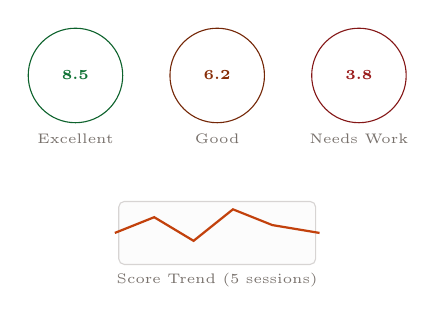
\begin{tikzpicture}[
  >=Stealth,
]

\node[draw=success!60!black, circle, minimum size=1.2cm] (r1) at (0, 2) {};
\node[font=\tiny\bfseries, text=success!70!black] at (0, 2) {8.5};

\node[draw=accent!60!black, circle, minimum size=1.2cm] (r2) at (1.8, 2) {};
\node[font=\tiny\bfseries, text=accent!70!black] at (1.8, 2) {6.2};

\node[draw=err!60!black, circle, minimum size=1.2cm] (r3) at (3.6, 2) {};
\node[font=\tiny\bfseries, text=err!70!black] at (3.6, 2) {3.8};

\node[font=\tiny, text=txt2] at (0, 1.2) {Excellent};
\node[font=\tiny, text=txt2] at (1.8, 1.2) {Good};
\node[font=\tiny, text=txt2] at (3.6, 1.2) {Needs Work};

\node[draw=txt2!30, fill=txt2!2, rounded corners=2pt, minimum width=2.5cm, minimum height=0.8cm] (spark) at (1.8, 0) {};
\draw[thick, color=accent] (0.5, 0) -- (1.0, 0.2) -- (1.5, -0.1) -- (2.0, 0.3) -- (2.5, 0.1) -- (3.1, 0);
\node[font=\tiny, text=txt2] at (1.8, -0.6) {Score Trend (5 sessions)};

\end{tikzpicture}
\caption{Score visualization with color-coded rings and sparkline trend charts.}
\label{fig:score}
\end{figure}

% ══════════════════════════════════════════════════════════
\section{Discussion}
\label{sec:discussion}

\subsection{Design Trade-offs}

Several deliberate trade-offs were made during development:

\begin{enumerate}[leftmargin=*, label=(\Roman*)]
  \item \textbf{No client-side router:} Using a \texttt{screen} state variable instead of URL-based navigation simplifies state management but prevents deep linking, browser back-button support, and shareable URLs for specific screens.
  \item \textbf{Single-component state:} All 18 state variables live in \texttt{AppInner}, avoiding prop drilling complexity but creating a large component ($\sim$357 lines) that re-renders on any state change.
  \item \textbf{Static content database:} Embedding questions in the bundle ensures instant availability but limits the question pool to 36 static items. Custom mode mitigates this by generating questions dynamically.
  \item \textbf{localStorage only:} No backend complexity, but session history is device-bound and lost on cache clear. No cross-device sync is possible.
  \item \textbf{Free AI model:} Using NVIDIA Nemotron 120B via OpenRouter's free tier eliminates cost but introduces potential rate limits and model availability risks.
\end{enumerate}

\subsection{Limitations}

The current implementation has several limitations. No user accounts or cross-device synchronization. No adaptive difficulty---question selection is random rather than performance-based. No exportable session reports beyond the browser print dialog. Custom mode requires AI generation, adding latency and an external API dependency. Voice input accuracy varies across browsers and hardware.

\subsection{Future Directions}

Planned improvements include: adaptive question selection using evaluation scores to target weak areas, spaced repetition scheduling for concept review, multi-language support for global audiences, team practice mode with shared evaluation reports, and enhanced PWA features including background sync and push notifications for practice reminders.

% ══════════════════════════════════════════════════════════
\section{Conclusion}
\label{sec:conclusion}

TeachLoop demonstrates that effective AI-assisted communication practice can be delivered with a minimal, client-side-first architecture. By combining a curated content database (36 questions, 108 hint sets), structured AI evaluation (5-dimension scoring), and a craft-oriented design system (3 themes, Perfect Fourth typography, grain textures), the platform provides actionable feedback on \emph{how} engineers explain technical concepts. The key architectural decision---a single API route proxying to a free LLM with localStorage persistence---eliminates backend infrastructure while maintaining a polished user experience. The progressive hint system, grounded in scaffolding theory, provides entry points for users at different skill levels. Future work will focus on adaptive difficulty and spaced repetition to improve long-term learning outcomes.

\balance

\begin{thebibliography}{9}

\bibitem{deeplearning}
DeepLearning.AI, ``Communicating with AI: Technical Explanations,'' DeepLearning.AI Short Courses, 2024. [Online]. Available: https://www.deeplearning.ai

\bibitem{vygotsky}
L.\,S. Vygotsky, \emph{Mind in Society: The Development of Higher Psychological Processes}. Cambridge, MA: Harvard Univ. Press, 1978.

\bibitem{vanlehn}
K. vanLehn, ``The relative effectiveness of human tutoring, intelligent tutoring systems, and other tutoring systems,'' \emph{Educational Psychologist}, vol. 46, no. 4, pp. 197--221, 2011.

\bibitem{leitner}
S. Leitner, \emph{So lernt man lernen}. Freiburg: Herder, 1972.

\bibitem{auto}
A.\,C. Graesser et al., ``Autotutor: A tutor with dialogue in natural language,'' \emph{Behavior Research Methods, Instruments, \& Computers}, vol. 36, no. 2, pp. 303--312, 2004.

\end{thebibliography}

\end{document}
